\documentclass[11pt, a4paper]{article}
\usepackage[a4paper, margin = 0.7in]{geometry}
\usepackage{graphicx}
\usepackage{amsmath}
\usepackage{listings}
\usepackage{url}

\title{EE2703 Assignment 7}
\author{Aman Kumar EE19B066}
\date{May 10, 2021}

\begin{document}

\maketitle

\section{Introduction}
This week's assignment involves the analysis of filters using laplace transforms. Sympy is a tool we use in the process to handle our requirements in solving Modified Nodal Analysis equations using symbolic algebra.
We also use scipy's signal toolbox to analyse the two filters for different inputs.
\section{The Assignment}
\subsection{The Low pass filter}
    The low pass filter given generates the following Modified Nodal Analysis Matrix:
    \[
    \begin{bmatrix}
        0   & 0 & 1  & -1/G \\
        \frac{-1}{sR_2C_2}  & 1 & 0 & 0\\
        0  & -G & G & 1 \\
        \frac{-1}{R_1} - \frac{1}{R_2} - sC_1 & \frac{1}{R_2} & 0 & sC_1
    \end{bmatrix}
    \begin{bmatrix}
        V_1\\
        V_p\\
        V_m \\
        V_o
    \end{bmatrix}
    =
    \begin{bmatrix}
        0 \\
        0 \\
        0 \\
        \frac{-V_i(s)}{R_1} \\
        
    \end{bmatrix}
    \]
    The python function \textit{lowpass()} makes the matrices \textbf{A} and \textbf{b} and solves them to get the solution vector \textbf{V}. It returns all these three matirces. Its magnitude response is plotted in Figure 1.
    \begin{verbatim}
def lowpass(r1,r2,c1,c2,g,vi):
    s = sp.symbols('s')
    #Creating the "A" matrix
    A = sp.Matrix([[0,0,1,-1/g],\
                   [-1/(1+s*r2*c2),1,0,0],\
                   [0,-g,g,1],\
                   [-1/r1-1/r2-s*c1,+1/r2,0,+s*c1]])
    #Creating the "b" matrix
    b = sp.Matrix([0,0,0,-vi/r1])
    V = A.inv()*b                 #Solving for V
    return(A,b,V)
    \end{verbatim}
\subsection{The High pass filter}
    The high pass filter given generates the following Modified Nodal Analysis Matrix:
    \[
    \begin{bmatrix}
        0   & 1 & 0  & -1/G \\
        \frac{-sC_2R_3}{1+sC_2R_3}  & 0 & 1 & 0\\
        0  & -G & G & 1 \\
        s(C_1+C_2) + \frac{1}{R_1}  & 0 & -sC_2 & \frac{-1}{R_1}
    \end{bmatrix}
    \begin{bmatrix}
        V_1\\
        V_p\\
        V_m \\
        V_o
    \end{bmatrix}
    =
    \begin{bmatrix}
        0 \\
        0 \\
        0 \\
        V_i(s)sC_1 \\
        
    \end{bmatrix}
    \]
    The python function \textit{highpass()} makes the matrices \textbf{A} and \textbf{b} and solves them to get the solution vector \textbf{V}. It returns all these three matirces. Its magnitude response is plotted in Figure 2.
    \begin{verbatim}
def highpass(r1,r3,c1,c2,g,vi):
    s = sp.symbols('s')
    #Creating the "A" matrix
    A = sp.Matrix([[0,0,1,-1/g],\
                  [-(s*r3*c2)/(1+s*r3*c2),1,0,0],\
                  [0,-g,g,1],\
                  [1/r1+s*(c1+c2),-s*c2,0,-1/r1]])
    #Creating the "b" matrix
    b = sp.Matrix([0,0,0,vi*s*c1])
    V = A.inv()*b                 #Solving for V
    return(A,b,V)
    \end{verbatim}
\subsection{Magnitude response}
    After solving the matrix equation, we have the symbolic expression for $V_o$. To plot the magnitude response I have defined a function - \textit{Magnitude\_response($V_o$)}:
    \begin{verbatim}
def Magnitude_response(Vo):
    s = sp.symbols('s')
    f = sp.lambdify(s,Vo,"numpy")
    p.xlabel("$\u03C9$")             #u03C9 is unicode for omega(w)
    p.loglog(w,abs(f(ss)),label="$|Vo(j\u03C9)|$")
    p.legend()
    p.grid(True)
    p.show()

A1,b1,V1 = lowpass(10000,10000,1e-9,1e-9,1.586,1)
A2,b2,V2 = highpass(10000,10000,1e-9,1e-9,1.586,1)
Vo_LP1 = V1[3].simplify()
Vo_HP1 = V2[3].simplify()
    \end{verbatim}
    \begin{figure}[!h]
        \centering
        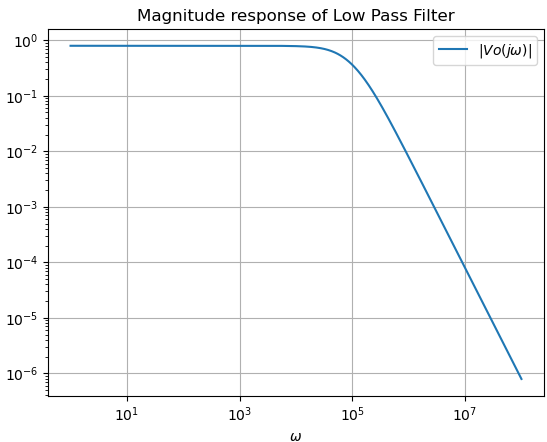
\includegraphics[scale=0.67]{Figure 1.png}
        \caption{Magnitude response of LPF}
        \label{fig:Figure 1}
    \end{figure}
    \begin{figure}[!h]
        \centering
        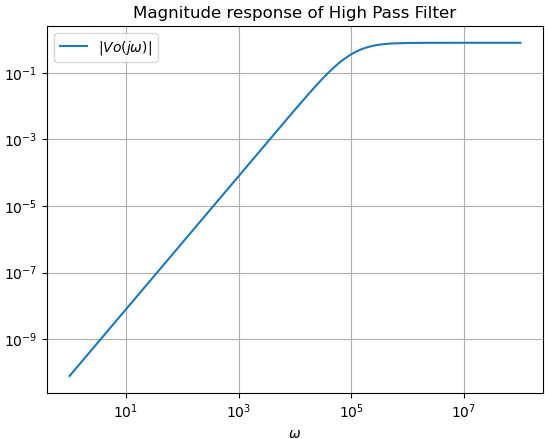
\includegraphics[scale=0.67]{Figure 2.png}
        \caption{Magnitude response of HPF}
        \label{fig:Figure 2}
    \end{figure}
\subsection{Getting the Transfer functions}
    After the solving the matrix equation, we get the \textit{V} vector. The output voltage $V_o$ is the last element in it. i.e. V[$3$]. But this expression is a sympy symbolic expression. So what I have done is, I have extracted the coefficients of both the numerator and denominator polynomials and defined the transfr fuunction using \textit{scipy.signal.lti} and then used it to get the tie responses of different inputs. The function used for extracting the coefficients: 
    \begin{verbatim}
def get_coeffs(expr):
    num,den = expr.as_numer_denom()     #num, den are numerator and
                                        #denominator polynomials
    return[sp.Poly(num,s).all_coeffs(),sp.Poly(den,s).all_coeffs()] 
    \end{verbatim}
    Calculting the coefficients of numerator and denominator polynomials for the transfer function of the Low Pass Filter.
    \begin{verbatim}
n,d = get_coeffs(Vo_LP1)
n_coeff,d_coeff = p.array(n,dtype="float"),p.array(d,dtype="float")
H_LP = sg.lti(n_coeff,d_coeff)          #Defining the transfer fucntion of LPF
    \end{verbatim}
    Calculting the coefficients of numerator and denominator polynomials for the transfer function of the High Pass Filter.
    \begin{verbatim}
n,d = get_coeffs(Vo_HP1)
n_coeff,d_coeff = p.array(n,dtype="float"),p.array(d,dtype="float")
H_HP = sg.lti(n_coeff,d_coeff)          #Defining the transfer fucntion of HPF
    \end{verbatim}
\subsection{Step response}
    Since, the transfer functions of both the LPF and HPF have already been evaluated, we just have to simulate them with the \textit{unit step function} as input i.e. $V_{in}$. I have defined a function \textit{Response(H,t,$V_{in}$)} that takes in three arguments - Transfer function, time vector and $V_{in}$ and plots the time response i.e. $V_o$. The following is the code used to plot(some unimportant parts omitted).
    \begin{verbatim}
def Response(H,t,Vin):
    
       t,Vo,svec = sg.lsim(H,Vin,t)      #Finding time response of H to Vin(t) 
       p.plot(t,Vo,label="Vout")
       p.xlabel("$t$")
       p.ylabel("$Vo$")
       p.grid(True)
       p.legend()
       p.show()

Vin1 = p.heaviside(t,1)          #Unit step function
Response(H_LP,t,Vin1)
Response(H_HP,t,Vin1)
    \end{verbatim}
    \begin{figure}[!h]
        \centering
        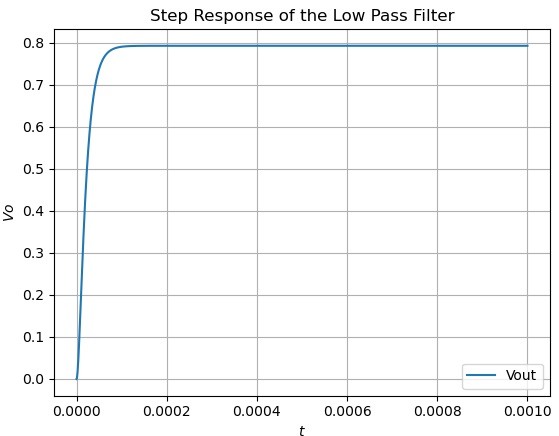
\includegraphics[scale = 0.65]{Figure 3.png}
        \caption{Step response of the LPF}
        \label{fig:Figure 3}
    \end{figure}
    \begin{figure}[!h]
        \centering
        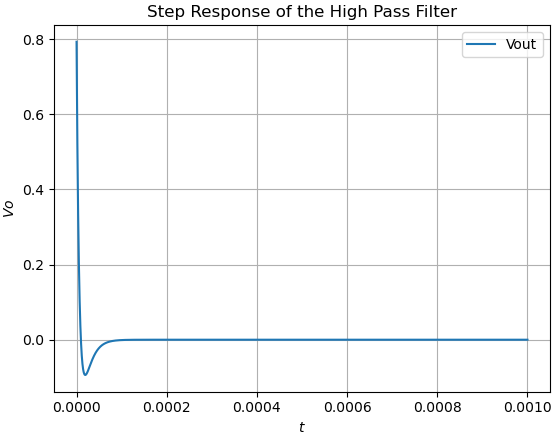
\includegraphics[scale = 0.65]{Figure 4.png}
        \caption{Step response of the HPF}
        \label{fig:Figure 4}
    \end{figure}
\subsection{Response to $v_i(t)$ = ($sin(2000\pi t)$ + $cos(2e6\pi t$))$u(t)$}
    So this is the sum of two different sinusoids of very different frequencies, one is a low frequency i.e. $2000$ and another $2*10^6$. So when we give this to LPF, we expect to see only the low frequency part in the output. Similarly, we expect to see only high frequency part in the output in case of HPF. Python code-
    \begin{verbatim}
Vin2 = (p.sin(2e3*p.pi*t) + p.cos(2e6*p.pi*t))*p.heaviside(t,1)

Response(H_LP,t,Vin2)                   #Plotting for t=0 to t=1ms
Response(H_HP,t[:201],Vin2[:201])       #Plotting for t=0 to t=20µs because the
                                        #high frequency componenet has frequency 2e6
    \end{verbatim}
    \begin{figure}[!h]
        \centering
        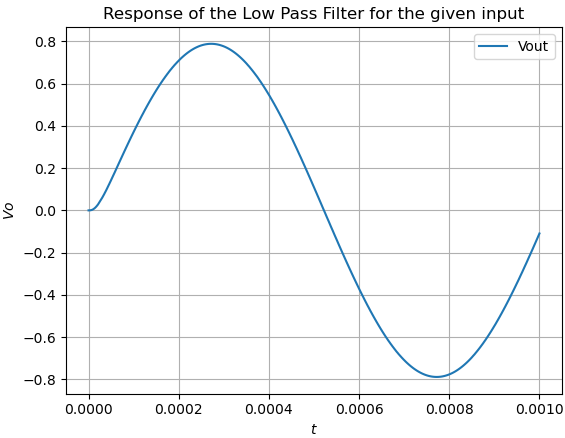
\includegraphics[scale = 0.65]{Figure 5.png}
        \caption{Response of the LPF}
        \label{fig:Figure 5}
    \end{figure}
    \begin{figure}[!h]
        \centering
        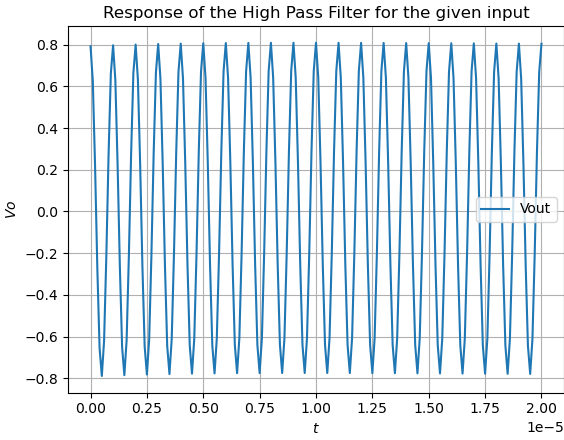
\includegraphics[scale = 0.65]{Figure 6.png}
        \caption{Response of the HPF}
        \label{fig:Figure 6}
    \end{figure}
    The results are as expected, the LPF allows only $sin(2000\pi t)$ and blocks the other part. Similarly, the HPF allows $cos(2e6\pi t)$ and blocks the other.
\subsection{Response of the High Pass filter to a damped sinusoid}
    I have used two damped sinusoids, one low frequency and the other high frequency.
    \begin{equation*}
        V_{damp1} = cos(10^6t).e^{-3000t}
    \end{equation*}
    \begin{equation*}
        V_{damp2} = cos(100t).e^{-3000t}
    \end{equation*}
    \begin{verbatim}
damp1 = p.cos(1e6*t)*p.exp(-3000*t)    #High frequency damped sinusoid       
damp2 = p.cos(100*t)*p.exp(-3000*t)    #Low frequency damped sinusoid
Response(H_HP,t,damp1)
Response(H_HP,t,damp2)
    \end{verbatim}
    \begin{figure}[!h]
        \centering
        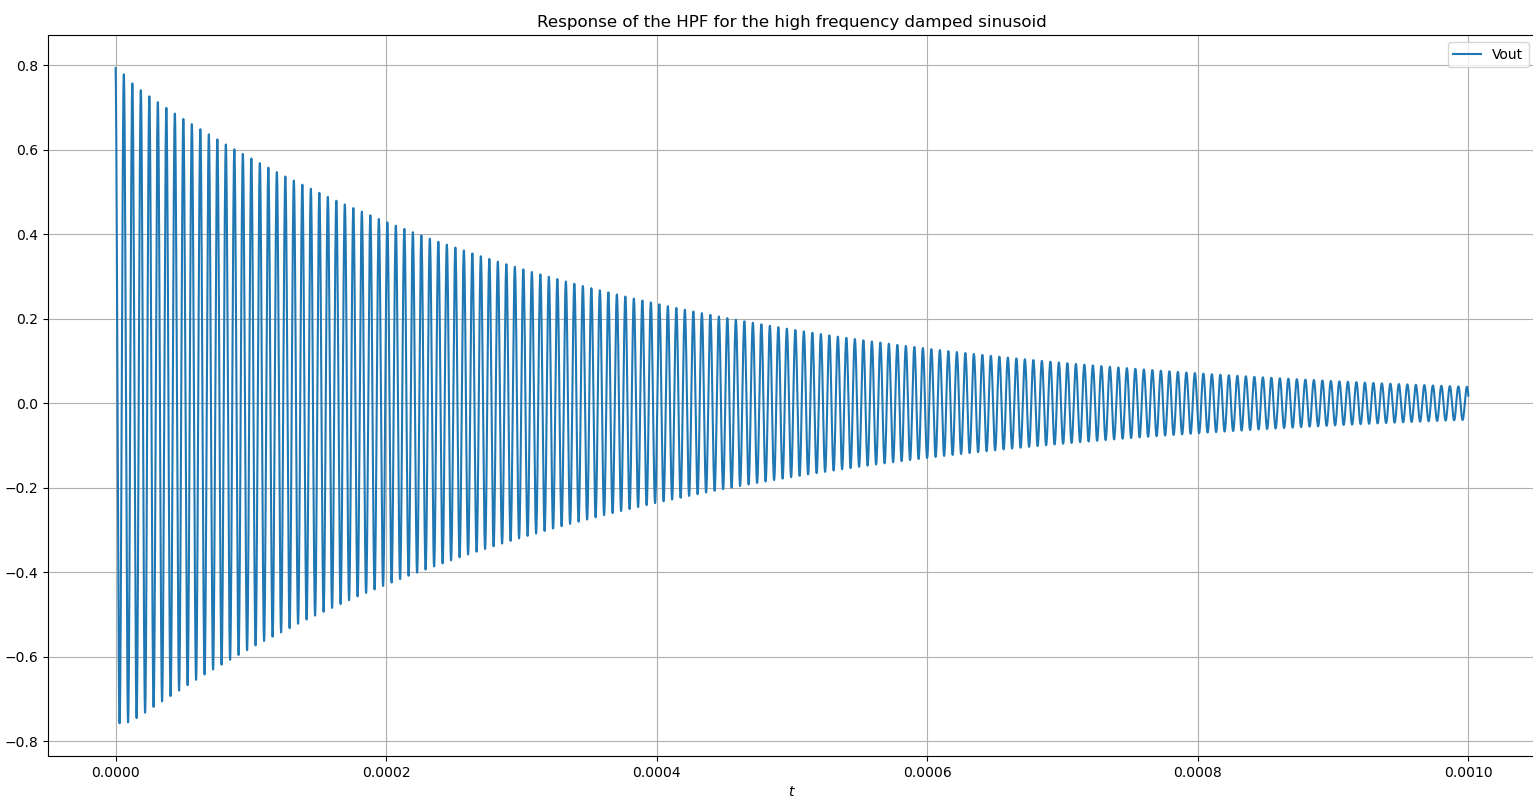
\includegraphics[scale = 0.43]{Figure 7.png}
        \caption{Response to $V_{damp1}$}
        \label{fig:Figure 7}
    \end{figure}
    \begin{figure}[!h]
        \centering
        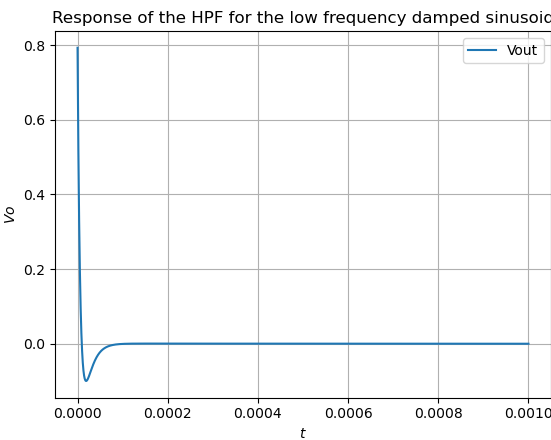
\includegraphics[scale = 0.65]{Figure 8.png}
        \caption{Response to $V_{damp2}$}
        \label{fig:Figure 8}
    \end{figure}
    Here also, we can see that the high frequency damped sinusoid is allowed to pass, but the low frequency damped sinusoid is blocked. It looks almost identical to the step response.
\section{Conclusion}
    In this assignment we have learned a very powerful tool in python that is \textit{symbolic algebra}. This sympy module helped us to analyse these two complicated circuits analytically and solving there node equations. We also learned the use of Laplace transforms in circuit analysis.
    
    We also used the \textit{signal toolbox} again in this assignment to get the time responses and defining the transfer functions. Thus, the signal tool box for scipy along with the sympy module is a very powerful tool for analysing and solving complex circuits such as the ones in this assignment.
\end{document}
